% Options for packages loaded elsewhere
\PassOptionsToPackage{unicode}{hyperref}
\PassOptionsToPackage{hyphens}{url}
%
\documentclass[
]{article}
\usepackage{lmodern}
\usepackage{amssymb,amsmath}
\usepackage{ifxetex,ifluatex}
\ifnum 0\ifxetex 1\fi\ifluatex 1\fi=0 % if pdftex
  \usepackage[T1]{fontenc}
  \usepackage[utf8]{inputenc}
  \usepackage{textcomp} % provide euro and other symbols
\else % if luatex or xetex
  \usepackage{unicode-math}
  \defaultfontfeatures{Scale=MatchLowercase}
  \defaultfontfeatures[\rmfamily]{Ligatures=TeX,Scale=1}
\fi
% Use upquote if available, for straight quotes in verbatim environments
\IfFileExists{upquote.sty}{\usepackage{upquote}}{}
\IfFileExists{microtype.sty}{% use microtype if available
  \usepackage[]{microtype}
  \UseMicrotypeSet[protrusion]{basicmath} % disable protrusion for tt fonts
}{}
\makeatletter
\@ifundefined{KOMAClassName}{% if non-KOMA class
  \IfFileExists{parskip.sty}{%
    \usepackage{parskip}
  }{% else
    \setlength{\parindent}{0pt}
    \setlength{\parskip}{6pt plus 2pt minus 1pt}}
}{% if KOMA class
  \KOMAoptions{parskip=half}}
\makeatother
\usepackage{xcolor}
\IfFileExists{xurl.sty}{\usepackage{xurl}}{} % add URL line breaks if available
\IfFileExists{bookmark.sty}{\usepackage{bookmark}}{\usepackage{hyperref}}
\hypersetup{
  pdftitle={R Notebook},
  hidelinks,
  pdfcreator={LaTeX via pandoc}}
\urlstyle{same} % disable monospaced font for URLs
\usepackage[margin=1in]{geometry}
\usepackage{color}
\usepackage{fancyvrb}
\newcommand{\VerbBar}{|}
\newcommand{\VERB}{\Verb[commandchars=\\\{\}]}
\DefineVerbatimEnvironment{Highlighting}{Verbatim}{commandchars=\\\{\}}
% Add ',fontsize=\small' for more characters per line
\usepackage{framed}
\definecolor{shadecolor}{RGB}{248,248,248}
\newenvironment{Shaded}{\begin{snugshade}}{\end{snugshade}}
\newcommand{\AlertTok}[1]{\textcolor[rgb]{0.94,0.16,0.16}{#1}}
\newcommand{\AnnotationTok}[1]{\textcolor[rgb]{0.56,0.35,0.01}{\textbf{\textit{#1}}}}
\newcommand{\AttributeTok}[1]{\textcolor[rgb]{0.77,0.63,0.00}{#1}}
\newcommand{\BaseNTok}[1]{\textcolor[rgb]{0.00,0.00,0.81}{#1}}
\newcommand{\BuiltInTok}[1]{#1}
\newcommand{\CharTok}[1]{\textcolor[rgb]{0.31,0.60,0.02}{#1}}
\newcommand{\CommentTok}[1]{\textcolor[rgb]{0.56,0.35,0.01}{\textit{#1}}}
\newcommand{\CommentVarTok}[1]{\textcolor[rgb]{0.56,0.35,0.01}{\textbf{\textit{#1}}}}
\newcommand{\ConstantTok}[1]{\textcolor[rgb]{0.00,0.00,0.00}{#1}}
\newcommand{\ControlFlowTok}[1]{\textcolor[rgb]{0.13,0.29,0.53}{\textbf{#1}}}
\newcommand{\DataTypeTok}[1]{\textcolor[rgb]{0.13,0.29,0.53}{#1}}
\newcommand{\DecValTok}[1]{\textcolor[rgb]{0.00,0.00,0.81}{#1}}
\newcommand{\DocumentationTok}[1]{\textcolor[rgb]{0.56,0.35,0.01}{\textbf{\textit{#1}}}}
\newcommand{\ErrorTok}[1]{\textcolor[rgb]{0.64,0.00,0.00}{\textbf{#1}}}
\newcommand{\ExtensionTok}[1]{#1}
\newcommand{\FloatTok}[1]{\textcolor[rgb]{0.00,0.00,0.81}{#1}}
\newcommand{\FunctionTok}[1]{\textcolor[rgb]{0.00,0.00,0.00}{#1}}
\newcommand{\ImportTok}[1]{#1}
\newcommand{\InformationTok}[1]{\textcolor[rgb]{0.56,0.35,0.01}{\textbf{\textit{#1}}}}
\newcommand{\KeywordTok}[1]{\textcolor[rgb]{0.13,0.29,0.53}{\textbf{#1}}}
\newcommand{\NormalTok}[1]{#1}
\newcommand{\OperatorTok}[1]{\textcolor[rgb]{0.81,0.36,0.00}{\textbf{#1}}}
\newcommand{\OtherTok}[1]{\textcolor[rgb]{0.56,0.35,0.01}{#1}}
\newcommand{\PreprocessorTok}[1]{\textcolor[rgb]{0.56,0.35,0.01}{\textit{#1}}}
\newcommand{\RegionMarkerTok}[1]{#1}
\newcommand{\SpecialCharTok}[1]{\textcolor[rgb]{0.00,0.00,0.00}{#1}}
\newcommand{\SpecialStringTok}[1]{\textcolor[rgb]{0.31,0.60,0.02}{#1}}
\newcommand{\StringTok}[1]{\textcolor[rgb]{0.31,0.60,0.02}{#1}}
\newcommand{\VariableTok}[1]{\textcolor[rgb]{0.00,0.00,0.00}{#1}}
\newcommand{\VerbatimStringTok}[1]{\textcolor[rgb]{0.31,0.60,0.02}{#1}}
\newcommand{\WarningTok}[1]{\textcolor[rgb]{0.56,0.35,0.01}{\textbf{\textit{#1}}}}
\usepackage{longtable,booktabs}
% Correct order of tables after \paragraph or \subparagraph
\usepackage{etoolbox}
\makeatletter
\patchcmd\longtable{\par}{\if@noskipsec\mbox{}\fi\par}{}{}
\makeatother
% Allow footnotes in longtable head/foot
\IfFileExists{footnotehyper.sty}{\usepackage{footnotehyper}}{\usepackage{footnote}}
\makesavenoteenv{longtable}
\usepackage{graphicx,grffile}
\makeatletter
\def\maxwidth{\ifdim\Gin@nat@width>\linewidth\linewidth\else\Gin@nat@width\fi}
\def\maxheight{\ifdim\Gin@nat@height>\textheight\textheight\else\Gin@nat@height\fi}
\makeatother
% Scale images if necessary, so that they will not overflow the page
% margins by default, and it is still possible to overwrite the defaults
% using explicit options in \includegraphics[width, height, ...]{}
\setkeys{Gin}{width=\maxwidth,height=\maxheight,keepaspectratio}
% Set default figure placement to htbp
\makeatletter
\def\fps@figure{htbp}
\makeatother
\setlength{\emergencystretch}{3em} % prevent overfull lines
\providecommand{\tightlist}{%
  \setlength{\itemsep}{0pt}\setlength{\parskip}{0pt}}
\setcounter{secnumdepth}{-\maxdimen} % remove section numbering

\title{R Notebook}
\author{}
\date{\vspace{-2.5em}}

\begin{document}
\maketitle

We have a sampling of \(n\) independent observation from a Gaussian
\emph{joint} distribution of dimension \(p\). These data are stored into
a matrix \(\mathbb{X} \in \mathbb{R}^{n\times p}\).

Given the matrix we want to get more clues about the unknown adjacency
matrix that models the DAG of the joint distribution that has generated
our observations.

This matrix is \(\mathbb{A}\) and it's a lower triangular matrix that
belongs to \(\mathbb{R}^{p\times p}\), and it's such that it has a 0 in
the position \((i,j)\) if \(j \not\in pa(X_i)\), else the value
represents the strength of the relationship that involves the two nodes.

We know how to model our observation, we know what \(\mathbb{A}\) means,
but how can we link the distribution of the j-th random variable
(remember that we have a p-dimensional random vector) to the matrix
\(\mathbb{A}\)? Well we can say that the j-th random variable \(X_j\)
can be computed as follows: \begin{equation}
  X_j = \sum_{k | k \neq j}\mathbb{A[j,k]\cdot X_k}+\epsilon_j
\end{equation} The Gaussian is in \(\epsilon\), in fact
\(\epsilon_j \sim N_1(0, \sigma^2)\).

So we have a model that depends from two parameters that are
\(\mathbb{A}\) and \(\sigma^2\). At this point we can proceed to the
things that are of interest for us.

Since we can obtain the distributions of the X from our parameters, we
want to discover our parameter starting from our observations, so the
problem is reduced to finding \(\theta = (\mathbb{A}, \sigma^2)\)
starting from \(\mathbb{X}\).

In order to do this we can use the log likelihood that's defined as
follows: \begin{equation}
  \mathcal{\ell}_n(\mathbb{A}, \sigma^2) \propto - \sum_{j=1}^p \left (\frac{1}{2\sigma^2} \sum_{i=1}^n \left( \mathbb{X}[i,j] - \sum_{k | k\neq j} \mathbb{A}[j,k]\cdot \mathbb{X}[i,k]\right)^2 + \frac{n}{2}ln\sigma^2 \right)
\end{equation} Let's enroll it: We have three sums that are, going from
the inner to the outer:

\begin{itemize}
\tightlist
\item
  \emph{inner}:
  \(\sum_{k \in [1,p] \setminus j} \mathbb{A}[j,k]\cdot \mathbb{X}[i,k]\)
  where we are computing the dot product from the weight that has the
  eventual edge that goes from \(k\) to \(j\) (scalar) and the value of
  the k-th random variable (\(X_k\)) in the i-th sample, and then
  summing all these values. This can be seen as a kind of weighted sum
  of the i-th sample where the weights are the influences that all the
  other random variables have over the k-th one, and as such it can be
  seen as a ``how much j is influenced by the other variables in the
  sample \(i\)''
\item
  \emph{middle}:
  \(\sum_{i=1}^n \left( \mathbb{X}[i,j] - \text{inner}\right )^2\) where
  for each of the i-th observation of the j-th random variable, we
  subtract the sum obtained in the inner that is a scalar, then summing
  all these values. We are subtracting the value of the j-th random
  variable in the sample i with the influence that the other random
  variables have had on \(j\), so we can interpret it as `how much j is
  distant from the value that should have accordingly with the other
  variables', then we compute the square of this difference. It can be
  interpreted as the euclidean distance from the vector of the n samples
  of j and the vector of the influences of all the other variables (the
  value that should have) over j.
\item
  \emph{outer}:
  \(\sum_{j=1}^p \frac{\text{middle}}{2\sigma^2} + \frac{n}{2}ln\sigma^2\)
  We sums up the value obtained from all the \(p\) random variables
  multiplied and summed with constants that are dependent from
  \(\sigma^2\)
\end{itemize}

Let's see it in code:

\begin{Shaded}
\begin{Highlighting}[]
\NormalTok{compute.middle =}\StringTok{ }\ControlFlowTok{function}\NormalTok{(X, A, j, p)\{}
  \CommentTok{# Finding the indexes K = \{k s.t. k is in [1,p]\textbackslash{}j\}}
\NormalTok{    K =}\StringTok{ }\KeywordTok{which}\NormalTok{((}\DecValTok{1}\OperatorTok{:}\NormalTok{p)}\OperatorTok{!=}\NormalTok{j)}
    \CommentTok{# in k we have the indexes of the row without j}
    
\NormalTok{    inners =}\StringTok{ }\KeywordTok{apply}\NormalTok{(X[, K] }\OperatorTok{*}\StringTok{ }\NormalTok{A[j, K], }\DecValTok{1}\NormalTok{, sum) }\CommentTok{# n length vector containing the inner sums for each i-th sample}
\NormalTok{    middle =}\StringTok{ }\KeywordTok{sum}\NormalTok{((X[, j] }\OperatorTok{-}\StringTok{ }\NormalTok{inners)}\OperatorTok{^}\DecValTok{2}\NormalTok{)  }\CommentTok{# as a matter of fact in the middle we are working on the j-th column}
    \KeywordTok{return}\NormalTok{(middle)}
\NormalTok{\}}

\NormalTok{log_likelihood =}\StringTok{ }\ControlFlowTok{function}\NormalTok{(X, A, sigma.square)\{}
\NormalTok{  n =}\StringTok{ }\KeywordTok{dim}\NormalTok{(X)[}\DecValTok{1}\NormalTok{]}
\NormalTok{  p =}\StringTok{ }\KeywordTok{dim}\NormalTok{(X)[}\DecValTok{2}\NormalTok{]}
  \KeywordTok{return}\NormalTok{(}\OperatorTok{-}\KeywordTok{sum}\NormalTok{(}\KeywordTok{sapply}\NormalTok{(}\DecValTok{1}\OperatorTok{:}\NormalTok{p, }\ControlFlowTok{function}\NormalTok{(j) (}\KeywordTok{compute.middle}\NormalTok{(X,A,j,p)}\OperatorTok{/}\NormalTok{(}\DecValTok{2}\OperatorTok{*}\NormalTok{sigma.square)}\OperatorTok{+}\NormalTok{(n}\OperatorTok{/}\DecValTok{2}\OperatorTok{*}\KeywordTok{log}\NormalTok{(sigma.square))))))}
\NormalTok{\}}
\end{Highlighting}
\end{Shaded}

Since MLEdag computes for us the estimate of the matrix \(\mathbb{A}\)
and the matrix \(\mathbb{X}\) is what we have, given that it's our
observation, we can optimize the log likelihood in order to retrieve
sigma, so it'll be the sigma.MLE

\begin{Shaded}
\begin{Highlighting}[]
\NormalTok{sigma.MLE =}\StringTok{ }\ControlFlowTok{function}\NormalTok{(X, A)}
  \KeywordTok{return}\NormalTok{(}
    \KeywordTok{optim}\NormalTok{(}
      \DataTypeTok{par=}\KeywordTok{c}\NormalTok{(}\FloatTok{0.01}\NormalTok{),}
      \DataTypeTok{fn=}\ControlFlowTok{function}\NormalTok{(sigma.sq)}
        \KeywordTok{log_likelihood}\NormalTok{(X,A, sigma.sq),}
      \DataTypeTok{method=}\KeywordTok{c}\NormalTok{(}\StringTok{"Brent"}\NormalTok{),}
      \DataTypeTok{lower =} \DecValTok{0}\NormalTok{,}
      \DataTypeTok{upper =} \DecValTok{10000}\NormalTok{,}
            \DataTypeTok{control =} \KeywordTok{list}\NormalTok{(}\DataTypeTok{fnscale =} \DecValTok{-1}\NormalTok{)}
\NormalTok{    )}
\NormalTok{  )}
\end{Highlighting}
\end{Shaded}

According with
\href{https://elearning.uniroma1.it/pluginfile.php/1112893/mod_assign/introattachment/0/Likelihood\%20Ratio\%20Tests\%20for\%20a\%20Large\%20Directed\%20Acyclic\%20Graph.pdf?forcedownload=1}{Chunlin
Li Et. al} we can also aproximate \(\sigma^2\) with: \begin{equation}
  \hat{\sigma}^2 = (np)^{-1} \sum_{j=1}^p \sum_{i=1}^n\left ( \mathbb{X}[i,j] - \sum_{k | k\neq j} \mathbb{A}[j,k]\cdot \mathbb{X}[i,k] \right ) ^2
\end{equation}

In code we have:

\begin{Shaded}
\begin{Highlighting}[]
\NormalTok{sigma.estimator =}\StringTok{ }\ControlFlowTok{function}\NormalTok{(X, A)\{}
\NormalTok{  n =}\StringTok{ }\KeywordTok{dim}\NormalTok{(X)[}\DecValTok{1}\NormalTok{]}
\NormalTok{  p =}\StringTok{ }\KeywordTok{dim}\NormalTok{(X)[}\DecValTok{2}\NormalTok{]}
  \KeywordTok{return}\NormalTok{(}\KeywordTok{sum}\NormalTok{(}\KeywordTok{sapply}\NormalTok{(}\DecValTok{1}\OperatorTok{:}\NormalTok{p, }\ControlFlowTok{function}\NormalTok{(j)}\KeywordTok{compute.middle}\NormalTok{(X,A,j, p)))}\OperatorTok{/}\NormalTok{(n}\OperatorTok{*}\NormalTok{p))}
\NormalTok{\}}
\end{Highlighting}
\end{Shaded}

\hypertarget{constrained-likelihood-ratio-test}{%
\subsection{Constrained Likelihood Ratio
Test}\label{constrained-likelihood-ratio-test}}

Since we can now approximate sigma and \(\mathbb{A}\) starting from
\(\mathbb{X}\), we can now run a constrained likelihood ratio test, in
order to test the existence of directed links between specific nodes or
directed pathways. The choice to reject the \(H_0\) hypothesis in the
two tests are made based on one of these two values:

\begin{itemize}
\tightlist
\item
  \(U_n\) for the \textbf{split} likelihood ratio
\item
  \(W_n\) for the \textbf{cross-fit} likelihood ratio
\end{itemize}

The main idea behind the computation of these two metrics is that when
we want the \textbf{constrained version} of \(\mathbb{A}\) we'll pass
into the \texttt{MLEdag} function the observation matrix, a matrix \(D\)
that is the matrix representation of the set of linkages \(F\) and is
such that has 1 only in the coordinates \((i, j) \in F\) and some other
numerical parameters. We'll compute over the entire observation the
estimate of \(\mathbb{A}\) with this function and we'll take the A.H0
result for the constrained version, and A.H1 for the unconstrained one.
Once we have the \(\mathbb{A}\) matrices, it's trivial to find the
estimates for the \(\sigma^2\) simply by using the function
\texttt{sigma.estimator} described above. In this specific case we'll
compute these estimates over the training part of \(\mathbb{X}\) for the
\textbf{constrained version} and over the test part for the other one.
At this point we have \(\hat{\theta}_0^{tr}\) and \(\hat{\theta}^{te}\)
to compute the \(U_n\) value and, consequently, the \(W_n\), but in both
cases we'll use their \emph{logarithmic version}.

We want to highlight that for the pathway test we also need to compute
not only the \(\theta\) that maximizes the likelihood but also we need
to find the right value of sparsity that maximizes it, so there will be
one more step in the computation, but the main idea remains the same.

\begin{Shaded}
\begin{Highlighting}[]
\NormalTok{compute.middle =}\StringTok{ }\ControlFlowTok{function}\NormalTok{(X,A,j, p)\{}
  \CommentTok{# Finding the indexes K = \{k s.t. k is in [1,p]\textbackslash{}j\}}
\NormalTok{  K =}\StringTok{ }\KeywordTok{which}\NormalTok{((}\DecValTok{1}\OperatorTok{:}\NormalTok{p)}\OperatorTok{!=}\NormalTok{j)}
  \CommentTok{# in k we have the indexes of the row without j}
  
\NormalTok{  inners =}\StringTok{ }\KeywordTok{apply}\NormalTok{(X[, K] }\OperatorTok{*}\StringTok{ }\NormalTok{A[j, K], }\DecValTok{1}\NormalTok{, sum) }\CommentTok{# n length vector containing the inner sums for each i-th sample}
\NormalTok{  middle =}\StringTok{ }\KeywordTok{sum}\NormalTok{((X[, j] }\OperatorTok{-}\StringTok{ }\NormalTok{inners)}\OperatorTok{^}\DecValTok{2}\NormalTok{)  }\CommentTok{# as a matter of fact in the middle we are working on the j-th column}
  \KeywordTok{return}\NormalTok{(middle)}
\NormalTok{\}}

\NormalTok{sigma.estimator =}\StringTok{ }\ControlFlowTok{function}\NormalTok{(X, A)\{}
\NormalTok{  n =}\StringTok{ }\KeywordTok{dim}\NormalTok{(X)[}\DecValTok{1}\NormalTok{]}
\NormalTok{  p =}\StringTok{ }\KeywordTok{dim}\NormalTok{(X)[}\DecValTok{2}\NormalTok{]}
  \KeywordTok{return}\NormalTok{(}\KeywordTok{sum}\NormalTok{(}\KeywordTok{sapply}\NormalTok{(}\DecValTok{1}\OperatorTok{:}\NormalTok{p, }\ControlFlowTok{function}\NormalTok{(j)}\KeywordTok{compute.middle}\NormalTok{(X,A,j, p)))}\OperatorTok{/}\NormalTok{(n}\OperatorTok{*}\NormalTok{p))}
\NormalTok{\}}

\NormalTok{log_likelihood =}\StringTok{ }\ControlFlowTok{function}\NormalTok{(X, A, sigma.square)\{}
\NormalTok{  n =}\StringTok{ }\KeywordTok{dim}\NormalTok{(X)[}\DecValTok{1}\NormalTok{]}
\NormalTok{  p =}\StringTok{ }\KeywordTok{dim}\NormalTok{(X)[}\DecValTok{2}\NormalTok{]}
  \KeywordTok{return}\NormalTok{(}\OperatorTok{-}\KeywordTok{sum}\NormalTok{(}\KeywordTok{sapply}\NormalTok{(}\DecValTok{1}\OperatorTok{:}\NormalTok{p, }\ControlFlowTok{function}\NormalTok{(j) (}\KeywordTok{compute.middle}\NormalTok{(X,A,j,p)}\OperatorTok{/}\NormalTok{(}\DecValTok{2}\OperatorTok{*}\NormalTok{sigma.square)}\OperatorTok{+}\NormalTok{(n}\OperatorTok{/}\DecValTok{2}\OperatorTok{*}\KeywordTok{log}\NormalTok{(sigma.square))))))}
\NormalTok{\}}


\NormalTok{inner_LRT_function.paths =}\StringTok{ }\ControlFlowTok{function}\NormalTok{(X, X.tr, X.te, D, mu, alpha )\{}
  
  \CommentTok{# Computing all the A.h0 over the sparsity parameters 'k'}
\NormalTok{  A.mles =}\StringTok{ }\KeywordTok{lapply}\NormalTok{(}\DecValTok{1}\OperatorTok{:}\KeywordTok{sum}\NormalTok{(D), }\ControlFlowTok{function}\NormalTok{(mu)}\KeywordTok{MLEdag}\NormalTok{(X, }\DataTypeTok{D=}\NormalTok{D, }\DataTypeTok{tau=}\NormalTok{alpha, }\DataTypeTok{mu=}\NormalTok{mu, }\DataTypeTok{rho=}\FloatTok{1.2}\NormalTok{, }\DataTypeTok{trace_obj =}\NormalTok{ F))}
\NormalTok{  A.h0s  =}\StringTok{ }\KeywordTok{lapply}\NormalTok{(A.mles, }\ControlFlowTok{function}\NormalTok{(a)a}\OperatorTok{$}\NormalTok{A.H0)}
\NormalTok{  A.h1s  =}\StringTok{ }\KeywordTok{lapply}\NormalTok{(A.mles, }\ControlFlowTok{function}\NormalTok{(a)a}\OperatorTok{$}\NormalTok{A.H1)}
  
  \CommentTok{# For each A.h0 compute the associated sigma}
\NormalTok{  sigmas}\FloatTok{.0}\NormalTok{ =}\StringTok{ }\KeywordTok{t}\NormalTok{(}\KeywordTok{sapply}\NormalTok{(A.h0s, }\ControlFlowTok{function}\NormalTok{(a)}\KeywordTok{sigma.estimator}\NormalTok{(X.tr, a)))}
\NormalTok{  sigmas}\FloatTok{.1}\NormalTok{ =}\StringTok{ }\KeywordTok{t}\NormalTok{(}\KeywordTok{sapply}\NormalTok{(A.h1s, }\ControlFlowTok{function}\NormalTok{(a)}\KeywordTok{sigma.estimator}\NormalTok{(X.te, a)))}
  
  \CommentTok{# Computing the likelihoods of each pair (A.h0, sigma.h0)}
\NormalTok{  likelihoods}\FloatTok{.0}\NormalTok{ =}\StringTok{ }\KeywordTok{t}\NormalTok{(}\KeywordTok{sapply}\NormalTok{(}\DecValTok{1}\OperatorTok{:}\KeywordTok{length}\NormalTok{(sigmas}\FloatTok{.0}\NormalTok{), }\ControlFlowTok{function}\NormalTok{(idx)}\KeywordTok{log_likelihood}\NormalTok{(X.tr, A.h0s[[idx]], sigmas}\FloatTok{.0}\NormalTok{[idx])))}
\NormalTok{  likelihoods}\FloatTok{.1}\NormalTok{ =}\StringTok{ }\KeywordTok{t}\NormalTok{(}\KeywordTok{sapply}\NormalTok{(}\DecValTok{1}\OperatorTok{:}\KeywordTok{length}\NormalTok{(sigmas}\FloatTok{.1}\NormalTok{), }\ControlFlowTok{function}\NormalTok{(idx)}\KeywordTok{log_likelihood}\NormalTok{(X.tr, A.h1s[[idx]], sigmas}\FloatTok{.1}\NormalTok{[idx])))}
  
  \CommentTok{# Finding the idx that give us the maximum likelihood}
\NormalTok{  mle_idx}\FloatTok{.0}\NormalTok{ =}\StringTok{ }\KeywordTok{which}\NormalTok{(likelihoods}\FloatTok{.0}\OperatorTok{==}\KeywordTok{max}\NormalTok{(likelihoods}\FloatTok{.0}\NormalTok{))[}\DecValTok{1}\NormalTok{] }\CommentTok{# maximum likelihood over h0}
\NormalTok{  mle_idx}\FloatTok{.1}\NormalTok{ =}\StringTok{ }\KeywordTok{which}\NormalTok{(likelihoods}\FloatTok{.1}\OperatorTok{==}\KeywordTok{max}\NormalTok{(likelihoods}\FloatTok{.1}\NormalTok{))[}\DecValTok{1}\NormalTok{] }\CommentTok{# maximum likelihood over h0}
  
  \KeywordTok{return}\NormalTok{ (likelihoods}\FloatTok{.1}\NormalTok{[mle_idx}\FloatTok{.1}\NormalTok{]}\OperatorTok{-}\NormalTok{likelihoods}\FloatTok{.0}\NormalTok{[mle_idx}\FloatTok{.0}\NormalTok{])}
  \CommentTok{#return(list(U.n=exp(log_likelihood(X.tr, A, sigma.unconstrained)-likelihoods[mle_idx]), A.h0=A.h0s[[mle_idx]]))}
  
\NormalTok{\}}

\NormalTok{inner_LRT_function.links =}\StringTok{ }\ControlFlowTok{function}\NormalTok{(X, X.tr, X.te, D, mu, alpha)\{}
\NormalTok{  tmp =}\StringTok{ }\KeywordTok{MLEdag}\NormalTok{(}\DataTypeTok{X =}\NormalTok{ X, }\DataTypeTok{D =}\NormalTok{ D, }\DataTypeTok{tau =}\NormalTok{ alpha, }\DataTypeTok{mu =}\NormalTok{ mu, }
               \DataTypeTok{rho =} \FloatTok{1.2}\NormalTok{, }\DataTypeTok{trace_obj =} \OtherTok{FALSE}\NormalTok{)}
\NormalTok{  A.h0 =}\StringTok{ }\NormalTok{tmp}\OperatorTok{$}\NormalTok{A.H0}
\NormalTok{  A =}\StringTok{ }\NormalTok{tmp}\OperatorTok{$}\NormalTok{A.H1}
  
\NormalTok{  sigma.h0 =}\StringTok{ }\KeywordTok{sigma.estimator}\NormalTok{(X.tr, A.h0)}
\NormalTok{  sigma.unconstrained =}\StringTok{ }\KeywordTok{sigma.estimator}\NormalTok{(X.te, A)}
  
  \KeywordTok{return}\NormalTok{(}\KeywordTok{log_likelihood}\NormalTok{(X.tr, A, sigma.unconstrained)}\OperatorTok{-}\KeywordTok{log_likelihood}\NormalTok{(X.tr, A.h0, sigma.h0))}
\NormalTok{\}}

\NormalTok{log.LRT =}\StringTok{ }\ControlFlowTok{function}\NormalTok{(X,D, }\DataTypeTok{links=}\NormalTok{T, mu,alpha)\{}
\NormalTok{  n=}\KeywordTok{dim}\NormalTok{(X)[}\DecValTok{1}\NormalTok{]}
\NormalTok{  X.tr =}\StringTok{ }\NormalTok{X[}\DecValTok{1}\OperatorTok{:}\NormalTok{(n}\OperatorTok\DecValTok{2}\NormalTok{),]}
\NormalTok{  X.te =}\StringTok{ }\NormalTok{X[(n}\OperatorTok\DecValTok{2}\OperatorTok{+}\DecValTok{1}\NormalTok{)}\OperatorTok{:}\NormalTok{n,]}
  
  \ControlFlowTok{if}\NormalTok{(links)\{}
\NormalTok{    U_n =}\StringTok{ }\KeywordTok{inner_LRT_function.links}\NormalTok{(X, X.tr, X.te, D, mu, alpha)}
\NormalTok{    U_n.swap =}\StringTok{ }\KeywordTok{inner_LRT_function.links}\NormalTok{(X, X.te, X.tr, D, mu, alpha)}
\NormalTok{  \}}
  \ControlFlowTok{else}\NormalTok{\{}
\NormalTok{    U_n =}\StringTok{ }\KeywordTok{inner_LRT_function.paths}\NormalTok{(X, X.tr, X.te, D, mu, alpha)}
\NormalTok{    U_n.swap =}\StringTok{ }\KeywordTok{inner_LRT_function.paths}\NormalTok{(X, X.te, X.tr, D,mu, alpha)}
\NormalTok{  \}}
  \KeywordTok{return}\NormalTok{(}\KeywordTok{list}\NormalTok{(}\DataTypeTok{links =}\NormalTok{ links, }\DataTypeTok{U_n =}\NormalTok{ U_n, }\DataTypeTok{W_n =}\NormalTok{ (}\KeywordTok{log}\NormalTok{((}\KeywordTok{exp}\NormalTok{(U_n)}\OperatorTok{+}\KeywordTok{exp}\NormalTok{(U_n.swap))}\OperatorTok{/}\DecValTok{2}\NormalTok{))))}
\NormalTok{\}}
\end{Highlighting}
\end{Shaded}

\hypertarget{testing-the-functions}{%
\subsubsection{Testing the functions}\label{testing-the-functions}}

Since we have implemented the computation of these ratios we can now
test whether a sample comes from a distribution that has a specific set
of linkages (or directed pathway) and when it hasn't it. In order to
test our implementation we've built two functions, one for the linkages
problem and one for the path. In both cases we built a linkages matrix
\(D\) and we create an adjacency matrix \(\mathbb{A}\) that is built in
function of a parameter \(h0\) that indicates if we want that
\(\mathbb{A} \in H_0\) or not. It also considers the value of \(\alpha\)
in order to execute the test. As anticipated we're working on the
logarithmic version of \(U_n\) and \(W_n\) so we'll check whether they
are lower than \(-log(\alpha)\). We sums up the times that we reject the
null hypothesis and if we pass h0=True we'll check the percentage of
False discoveries, which is expected to be around the value of \(alpha\)
(actually it should be lower than it, but since it's a new and
experimental way to make these kind of tests, it's acceptable if we
don't achieve perfect results.). We can also check the percentage of
true negatives passing h0=False.

\begin{Shaded}
\begin{Highlighting}[]
\KeywordTok{library}\NormalTok{(cli)}
\end{Highlighting}
\end{Shaded}

\begin{verbatim}
## Warning: package 'cli' was built under R version 4.0.2
\end{verbatim}

\begin{Shaded}
\begin{Highlighting}[]
\KeywordTok{library}\NormalTok{(clrdag)}
\NormalTok{test_path =}\StringTok{ }\ControlFlowTok{function}\NormalTok{(}\DataTypeTok{m=}\FloatTok{1e2}\NormalTok{,}\DataTypeTok{h0=}\NormalTok{T, }\DataTypeTok{alpha =} \FloatTok{.05}\NormalTok{)\{}
  \CommentTok{# matrices parameters}
\NormalTok{  p =}\StringTok{ }\DecValTok{10}
\NormalTok{  n =}\StringTok{ }\DecValTok{100}
\NormalTok{  sparsity =}\StringTok{ }\DecValTok{2}\OperatorTok{/}\NormalTok{p}
  
  \CommentTok{# Building the linkages set}
\NormalTok{  D.pathway =}\StringTok{ }\KeywordTok{matrix}\NormalTok{(}\DecValTok{0}\NormalTok{, p,p)}
\NormalTok{  D.pathway[}\DecValTok{3}\NormalTok{, }\DecValTok{4}\NormalTok{]=}\DecValTok{1}
\NormalTok{  D.pathway[}\DecValTok{4}\NormalTok{, }\DecValTok{5}\NormalTok{]=}\DecValTok{1}
\NormalTok{  D.pathway[}\DecValTok{5}\NormalTok{, }\DecValTok{6}\NormalTok{]=}\DecValTok{1}
\NormalTok{  D.pathway[}\DecValTok{6}\NormalTok{, }\DecValTok{7}\NormalTok{]=}\DecValTok{1}
  \CommentTok{# Building A accordingly to h0}
\NormalTok{  A.pathway.hidden =}\StringTok{ }\KeywordTok{matrix}\NormalTok{(}\KeywordTok{rbinom}\NormalTok{(p}\OperatorTok{*}\NormalTok{p,}\DecValTok{1}\NormalTok{,sparsity)}\OperatorTok{*}\KeywordTok{sign}\NormalTok{(}\KeywordTok{runif}\NormalTok{(p}\OperatorTok{*}\NormalTok{p,}\DataTypeTok{min=}\OperatorTok{-}\DecValTok{1}\NormalTok{,}\DataTypeTok{max=}\DecValTok{1}\NormalTok{)),p,p)}
\NormalTok{  A.pathway.hidden[}\KeywordTok{upper.tri}\NormalTok{(A.pathway.hidden, }\DataTypeTok{diag =}\NormalTok{ T)] =}\StringTok{ }\DecValTok{0}
\NormalTok{  A.pathway.hidden[}\DecValTok{4}\NormalTok{,}\DecValTok{3}\NormalTok{]=}\KeywordTok{as.integer}\NormalTok{(}\OperatorTok{!}\NormalTok{h0)}
\NormalTok{  A.pathway.hidden[}\DecValTok{5}\NormalTok{,}\DecValTok{4}\NormalTok{]=}\DecValTok{0}
\NormalTok{  A.pathway.hidden[}\DecValTok{6}\NormalTok{,}\DecValTok{5}\NormalTok{]=}\DecValTok{0}
\NormalTok{  A.pathway.hidden[}\DecValTok{7}\NormalTok{,}\DecValTok{6}\NormalTok{]=}\DecValTok{0}
  
  \CommentTok{# Running the actual test}
\NormalTok{  out_U =}\StringTok{ }\DecValTok{0}
\NormalTok{  out_W =}\StringTok{ }\DecValTok{0}
  \KeywordTok{cli_progress_bar}\NormalTok{(}\StringTok{"Cleaning data"}\NormalTok{, }\DataTypeTok{total =}\NormalTok{ m)}
  \ControlFlowTok{for}\NormalTok{(i }\ControlFlowTok{in} \DecValTok{1}\OperatorTok{:}\NormalTok{m)\{}
\NormalTok{    X =}\StringTok{ }\KeywordTok{matrix}\NormalTok{( }\KeywordTok{rnorm}\NormalTok{(n}\OperatorTok{*}\NormalTok{p), n, p) }\OperatorTok\StringTok{ }\KeywordTok{t}\NormalTok{(}\KeywordTok{solve}\NormalTok{(}\KeywordTok{diag}\NormalTok{(p) }\OperatorTok{-}\StringTok{ }\NormalTok{A.pathway.hidden) )}
\NormalTok{    LRT =}\StringTok{ }\KeywordTok{log.LRT}\NormalTok{(X, D.pathway, }\DataTypeTok{links=}\NormalTok{F)}
    \ControlFlowTok{if}\NormalTok{(LRT}\OperatorTok{$}\NormalTok{links)}
      \KeywordTok{cat}\NormalTok{(}\StringTok{'ERRORE, chiamata LRT con links='}\NormalTok{, links,}\StringTok{'}\CharTok{\textbackslash{}n}\StringTok{'}\NormalTok{)}
\NormalTok{    out_U =}\StringTok{ }\NormalTok{out_U}\OperatorTok{+}\NormalTok{(LRT}\OperatorTok{$}\NormalTok{U_n}\OperatorTok{>-}\KeywordTok{log}\NormalTok{(alpha))}
\NormalTok{    out_W =}\StringTok{ }\NormalTok{out_W}\OperatorTok{+}\NormalTok{(LRT}\OperatorTok{$}\NormalTok{W_n}\OperatorTok{>-}\KeywordTok{log}\NormalTok{(alpha))}
    \KeywordTok{cli_progress_update}\NormalTok{()}
\NormalTok{  \}}
  \KeywordTok{cli_progress_done}\NormalTok{()}
  \KeywordTok{return}\NormalTok{(}\KeywordTok{list}\NormalTok{(}\DataTypeTok{U_n =}\NormalTok{ out_U}\OperatorTok{/}\NormalTok{m, }\DataTypeTok{W_n =}\NormalTok{ out_W}\OperatorTok{/}\NormalTok{m))}
\NormalTok{\}}

\NormalTok{test_link =}\StringTok{ }\ControlFlowTok{function}\NormalTok{(}\DataTypeTok{m=}\FloatTok{1e3}\NormalTok{, }\DataTypeTok{alpha=}\NormalTok{.}\DecValTok{05}\NormalTok{, }\DataTypeTok{h0=}\NormalTok{T)\{}
  \CommentTok{# matrices parameters}
\NormalTok{  p =}\StringTok{ }\DecValTok{10}
\NormalTok{  n=}\StringTok{ }\DecValTok{100}
\NormalTok{  sparsity =}\StringTok{ }\DecValTok{2}\OperatorTok{/}\NormalTok{p}
  
  \CommentTok{# Building the linkages set}
\NormalTok{  D.link =}\StringTok{ }\KeywordTok{matrix}\NormalTok{(}\DecValTok{0}\NormalTok{, p, p)}
\NormalTok{  D.link[}\DecValTok{2}\NormalTok{, }\DecValTok{1}\NormalTok{] =}\StringTok{ }\DecValTok{1}
\NormalTok{  D.link[}\DecValTok{6}\NormalTok{, }\DecValTok{3}\NormalTok{] =}\StringTok{ }\DecValTok{1}
\NormalTok{  D.link[}\DecValTok{10}\NormalTok{, }\DecValTok{9}\NormalTok{] =}\StringTok{ }\DecValTok{1}
  \CommentTok{# Building A accordingly to h0}
\NormalTok{  A.link.hidden =}\StringTok{ }\KeywordTok{matrix}\NormalTok{(}\KeywordTok{rbinom}\NormalTok{(p}\OperatorTok{*}\NormalTok{p,}\DecValTok{1}\NormalTok{,sparsity)}\OperatorTok{*}\KeywordTok{sign}\NormalTok{(}\KeywordTok{runif}\NormalTok{(p}\OperatorTok{*}\NormalTok{p,}\DataTypeTok{min=}\OperatorTok{-}\DecValTok{1}\NormalTok{,}\DataTypeTok{max=}\DecValTok{1}\NormalTok{)),p,p)}
\NormalTok{  A.link.hidden[}\KeywordTok{upper.tri}\NormalTok{(A.link.hidden, }\DataTypeTok{diag =}\NormalTok{ T)] =}\StringTok{ }\DecValTok{0}
\NormalTok{  A.link.hidden[}\DecValTok{2}\NormalTok{, }\DecValTok{1}\NormalTok{] =}\StringTok{ }\DecValTok{1}\CommentTok{#as.integer(!h0)}
\NormalTok{  A.link.hidden[}\DecValTok{6}\NormalTok{, }\DecValTok{3}\NormalTok{] =}\StringTok{ }\DecValTok{1}
\NormalTok{  A.link.hidden[}\DecValTok{10}\NormalTok{, }\DecValTok{9}\NormalTok{] =}\DecValTok{1}
  
  \CommentTok{# Running the actual test}
\NormalTok{  out_U =}\StringTok{ }\DecValTok{0}
\NormalTok{  out_W =}\StringTok{ }\DecValTok{0}
  \KeywordTok{cli_progress_bar}\NormalTok{(}\StringTok{"Cleaning data"}\NormalTok{, }\DataTypeTok{total =}\NormalTok{ m)}
  \ControlFlowTok{for}\NormalTok{(i }\ControlFlowTok{in} \DecValTok{1}\OperatorTok{:}\NormalTok{m)\{}
\NormalTok{    X =}\StringTok{ }\KeywordTok{matrix}\NormalTok{( }\KeywordTok{rnorm}\NormalTok{(n}\OperatorTok{*}\NormalTok{p), n, p) }\OperatorTok\StringTok{ }\KeywordTok{t}\NormalTok{(}\KeywordTok{solve}\NormalTok{(}\KeywordTok{diag}\NormalTok{(p) }\OperatorTok{-}\StringTok{ }\NormalTok{A.link.hidden) )}
\NormalTok{    LRT =}\StringTok{ }\KeywordTok{log.LRT}\NormalTok{(X, D.link, }\DataTypeTok{links=}\NormalTok{T)}
    \ControlFlowTok{if}\NormalTok{(}\OperatorTok{!}\NormalTok{LRT}\OperatorTok{$}\NormalTok{links)}
      \KeywordTok{cat}\NormalTok{(}\StringTok{'ERRORE, chiamata LRT con links='}\NormalTok{, links,}\StringTok{'}\CharTok{\textbackslash{}n}\StringTok{'}\NormalTok{)}
\NormalTok{    out_U =}\StringTok{ }\NormalTok{out_U}\OperatorTok{+}\NormalTok{(LRT}\OperatorTok{$}\NormalTok{U_n}\OperatorTok{>-}\KeywordTok{log}\NormalTok{(alpha))}
\NormalTok{    out_W =}\StringTok{ }\NormalTok{out_W}\OperatorTok{+}\NormalTok{(LRT}\OperatorTok{$}\NormalTok{W_n}\OperatorTok{>-}\KeywordTok{log}\NormalTok{(alpha))}
    \KeywordTok{cli_progress_update}\NormalTok{()}
\NormalTok{  \}}
  \KeywordTok{cli_progress_done}\NormalTok{()}
  \KeywordTok{return}\NormalTok{(}\KeywordTok{list}\NormalTok{(}\DataTypeTok{U_n=}\NormalTok{out_U}\OperatorTok{/}\NormalTok{m, }\DataTypeTok{W_n=}\NormalTok{out_W}\OperatorTok{/}\NormalTok{m))}
\NormalTok{\}}
\end{Highlighting}
\end{Shaded}

\hypertarget{part-3}{%
\subsection{PART 3}\label{part-3}}

Now let's check the size \(\alpha\) and the power \$ 1- \beta \$ of our
procedure.

Let's check the size and the power in the case of linkages-type test.

Starting from the size and noticing that the power is the proportion of
rejections we get by applying our test on M dataset generated from a
model \emph{compatible} with H0, we implemented the following
simulation:

\begin{Shaded}
\begin{Highlighting}[]
\CommentTok{### Parameters}
\KeywordTok{set.seed}\NormalTok{(}\DecValTok{2018}\NormalTok{)}
\NormalTok{p <-}\StringTok{ }\DecValTok{10}
\NormalTok{n <-}\StringTok{ }\DecValTok{200}
\NormalTok{M <-}\StringTok{ }\DecValTok{1000}

\CommentTok{### H0: F = \{ (p,2) \}, and A[F] = 0}
\NormalTok{D <-}\StringTok{ }\KeywordTok{matrix}\NormalTok{(}\DecValTok{0}\NormalTok{, p, p)}
\NormalTok{D[p,}\DecValTok{2}\NormalTok{] =}\StringTok{ }\DecValTok{1}

\CommentTok{### Adjacency Matrix >> Hub}
\CommentTok{# All connected to 1, NO EDGE between p-2 >> **COMPATIBLE** with H0}
\NormalTok{A      <-}\StringTok{ }\KeywordTok{matrix}\NormalTok{(}\DecValTok{0}\NormalTok{, p, p)     }
\NormalTok{A[, }\DecValTok{1}\NormalTok{] <-}\StringTok{ }\KeywordTok{sign}\NormalTok{( }\KeywordTok{runif}\NormalTok{( p, }\DataTypeTok{min =} \DecValTok{-1}\NormalTok{, }\DataTypeTok{max =} \DecValTok{1}\NormalTok{ ) )}
\NormalTok{A[}\DecValTok{1}\NormalTok{,}\DecValTok{1}\NormalTok{] <-}\StringTok{ }\DecValTok{0}

\CommentTok{# Simulation --------------------------------------------------------------}

\NormalTok{M=}\DecValTok{1000}
\NormalTok{cont=}\DecValTok{0}
\NormalTok{alpha=}\FloatTok{0.05}
\NormalTok{contU=}\DecValTok{0}
\NormalTok{contW=}\DecValTok{0}
\NormalTok{U_n <-}\StringTok{ }\KeywordTok{rep}\NormalTok{(}\OtherTok{NA}\NormalTok{, M)}
\NormalTok{W_n <-}\StringTok{ }\KeywordTok{rep}\NormalTok{(}\OtherTok{NA}\NormalTok{, M)}
\ControlFlowTok{for}\NormalTok{(i }\ControlFlowTok{in} \DecValTok{1}\OperatorTok{:}\NormalTok{M) \{}
\NormalTok{  X   <-}\StringTok{ }\KeywordTok{matrix}\NormalTok{( }\KeywordTok{rnorm}\NormalTok{(n}\OperatorTok{*}\NormalTok{p), n, p) }\OperatorTok\StringTok{ }\KeywordTok{t}\NormalTok{(}\KeywordTok{solve}\NormalTok{(}\KeywordTok{diag}\NormalTok{(p) }\OperatorTok{-}\StringTok{ }\NormalTok{A) )}
\NormalTok{  temp=}\KeywordTok{log.LRT}\NormalTok{(X,D, }\DataTypeTok{links=}\NormalTok{T,}\DataTypeTok{mu=}\FloatTok{1.2}\NormalTok{,}\DataTypeTok{alpha=}\NormalTok{alpha)}
\NormalTok{  U_n[i]=temp}\OperatorTok{$}\NormalTok{U_n}
\NormalTok{  W_n[i]=temp}\OperatorTok{$}\NormalTok{W_n}
  
  \ControlFlowTok{if}\NormalTok{ (U_n[i]}\OperatorTok{>}\KeywordTok{log}\NormalTok{(}\DecValTok{1}\OperatorTok{/}\NormalTok{alpha)) contU=contU}\OperatorTok{+}\DecValTok{1}
  \ControlFlowTok{if}\NormalTok{ (W_n[i]}\OperatorTok{>}\KeywordTok{log}\NormalTok{(}\DecValTok{1}\OperatorTok{/}\NormalTok{alpha)) contW=contW}\OperatorTok{+}\DecValTok{1}
\NormalTok{\}}

\KeywordTok{cat}\NormalTok{(}\StringTok{'alpha is equal to for U '}\NormalTok{, contU}\OperatorTok{/}\NormalTok{M,}\StringTok{'alpha is equal to for W'}\NormalTok{,contW}\OperatorTok{/}\NormalTok{M)}
\end{Highlighting}
\end{Shaded}

\begin{verbatim}
## alpha is equal to for U  0.049 alpha is equal to for W 0.053
\end{verbatim}

\begin{Shaded}
\begin{Highlighting}[]
\CommentTok{# 0.092 and 0.103}
\end{Highlighting}
\end{Shaded}

Our results are 0.092 for Un and 0.103 for Wn respectively.

Noticing that the power is the proportion of rejections we get by
applying our test on M dataset generated from a model \emph{NOT
compatible} with H0, we implemented the following simulation:

\begin{Shaded}
\begin{Highlighting}[]
\CommentTok{#Beta= the probability of failing to reject the null hypothesis when the null }
\CommentTok{# hypothesis is false}
\NormalTok{p=}\DecValTok{10}
\NormalTok{n=}\DecValTok{100}
\NormalTok{sparsity=}\DecValTok{2}\OperatorTok{/}\NormalTok{p}
\CommentTok{### H0: F = \{ (p,1) \}, and A[F] = 0}
\NormalTok{D <-}\StringTok{ }\KeywordTok{matrix}\NormalTok{(}\DecValTok{0}\NormalTok{, p, p)}
\NormalTok{D[}\DecValTok{2}\OperatorTok{:}\NormalTok{p,}\DecValTok{1}\NormalTok{]=}\DecValTok{1}
\NormalTok{D[}\DecValTok{3}\OperatorTok{:}\NormalTok{p,}\DecValTok{2}\NormalTok{]=}\DecValTok{1}

\CommentTok{### Adjacency Matrix >> Hub}
\CommentTok{# All connected to 1, NO EDGE between p-2 >> **NOT COMPATIBLE** with H0}
\CommentTok{#A      <- matrix(0, p, p)     }
\CommentTok{#A[2:p, 1] <- sign( runif( p-1, min = -1, max = 1 ) )}
\KeywordTok{set.seed}\NormalTok{(}\DecValTok{2018}\NormalTok{)}
\NormalTok{A=}\KeywordTok{matrix}\NormalTok{(}\KeywordTok{rbinom}\NormalTok{(p}\OperatorTok{*}\NormalTok{p,}\DecValTok{1}\NormalTok{,sparsity)}\OperatorTok{*}\KeywordTok{sign}\NormalTok{(}\KeywordTok{runif}\NormalTok{(p}\OperatorTok{*}\NormalTok{p,}\DataTypeTok{min=}\OperatorTok{-}\DecValTok{1}\NormalTok{,}\DataTypeTok{max=}\DecValTok{1}\NormalTok{)),p,p)}
\NormalTok{A[}\DecValTok{2}\NormalTok{,}\DecValTok{8}\NormalTok{]=}\DecValTok{1}
\NormalTok{A[}\DecValTok{5}\NormalTok{,}\DecValTok{6}\NormalTok{]=}\DecValTok{1}
\NormalTok{A[}\DecValTok{8}\NormalTok{,}\DecValTok{9}\NormalTok{]=}\DecValTok{1}
\NormalTok{A[}\DecValTok{2}\OperatorTok{:}\NormalTok{p,}\DecValTok{1}\NormalTok{]=}\DecValTok{1}
\NormalTok{A[}\DecValTok{3}\OperatorTok{:}\NormalTok{p,}\DecValTok{2}\NormalTok{]=}\DecValTok{1}

\CommentTok{# SIMULATION}
\NormalTok{contU=}\DecValTok{0}
\NormalTok{contW=}\DecValTok{0}
\NormalTok{alpha=}\FloatTok{0.05}
\NormalTok{M=}\DecValTok{1000}
\NormalTok{U_n <-}\StringTok{ }\KeywordTok{rep}\NormalTok{(}\OtherTok{NA}\NormalTok{, M)}
\NormalTok{W_n <-}\StringTok{ }\KeywordTok{rep}\NormalTok{(}\OtherTok{NA}\NormalTok{, M)}
\ControlFlowTok{for}\NormalTok{(i }\ControlFlowTok{in} \DecValTok{1}\OperatorTok{:}\NormalTok{M) \{}
\NormalTok{  X   <-}\StringTok{ }\KeywordTok{matrix}\NormalTok{( }\KeywordTok{rnorm}\NormalTok{(n}\OperatorTok{*}\NormalTok{p), n, p) }\OperatorTok\StringTok{ }\KeywordTok{t}\NormalTok{(}\KeywordTok{solve}\NormalTok{(}\KeywordTok{diag}\NormalTok{(p) }\OperatorTok{-}\StringTok{ }\NormalTok{A) )}
\NormalTok{  temp=}\KeywordTok{log.LRT}\NormalTok{(X,D, }\DataTypeTok{links=}\NormalTok{T,}\DataTypeTok{mu=}\FloatTok{1.2}\NormalTok{,}\DataTypeTok{alpha=}\NormalTok{alpha)}
\NormalTok{  U_n[i]=temp}\OperatorTok{$}\NormalTok{U_n}
\NormalTok{  W_n[i]=temp}\OperatorTok{$}\NormalTok{W_n}
  
  \ControlFlowTok{if}\NormalTok{ (U_n[i]}\OperatorTok{>}\KeywordTok{log}\NormalTok{(}\DecValTok{1}\OperatorTok{/}\NormalTok{alpha)) contU=contU}\OperatorTok{+}\DecValTok{1}
  \ControlFlowTok{if}\NormalTok{ (W_n[i]}\OperatorTok{>}\KeywordTok{log}\NormalTok{(}\DecValTok{1}\OperatorTok{/}\NormalTok{alpha)) contW=contW}\OperatorTok{+}\DecValTok{1}
\NormalTok{\}}

\KeywordTok{cat}\NormalTok{(}\StringTok{'1-beta is equal to for U: '}\NormalTok{, contU}\OperatorTok{/}\NormalTok{M,}\StringTok{'   ,1-beta is equal to for W:'}\NormalTok{,contW}\OperatorTok{/}\NormalTok{M)}
\end{Highlighting}
\end{Shaded}

\begin{verbatim}
## 1-beta is equal to for U:  0.734    ,1-beta is equal to for W: 0.848
\end{verbatim}

\begin{Shaded}
\begin{Highlighting}[]
\CommentTok{#1-beta is equal to for U:  0.969    ,1-beta is equal to for W: 0.991}
\end{Highlighting}
\end{Shaded}

that produce as results 0.969 for Un and 0.991 for Wn respectively.

Let's continue checking the size and the power for pathway-type test.

\begin{Shaded}
\begin{Highlighting}[]
\NormalTok{p =}\StringTok{ }\DecValTok{10}
\NormalTok{n =}\StringTok{ }\DecValTok{100}
\NormalTok{sparsity =}\StringTok{ }\DecValTok{2}\OperatorTok{/}\NormalTok{p}

\CommentTok{# Building the linkages set}
\NormalTok{D.pathway =}\StringTok{ }\KeywordTok{matrix}\NormalTok{(}\DecValTok{0}\NormalTok{, p,p)}
\NormalTok{D.pathway[}\DecValTok{3}\NormalTok{, }\DecValTok{4}\NormalTok{]=}\DecValTok{1}
\NormalTok{D.pathway[}\DecValTok{4}\NormalTok{, }\DecValTok{5}\NormalTok{]=}\DecValTok{1}
\NormalTok{D.pathway[}\DecValTok{5}\NormalTok{, }\DecValTok{6}\NormalTok{]=}\DecValTok{1}
\NormalTok{D.pathway[}\DecValTok{6}\NormalTok{, }\DecValTok{7}\NormalTok{]=}\DecValTok{1}
\CommentTok{# Building A accordingly to h0}
\NormalTok{A.pathway.hidden=}\KeywordTok{matrix}\NormalTok{(}\KeywordTok{rbinom}\NormalTok{(p}\OperatorTok{*}\NormalTok{p,}\DecValTok{1}\NormalTok{,sparsity)}\OperatorTok{*}\KeywordTok{sign}\NormalTok{(}\KeywordTok{runif}\NormalTok{(p}\OperatorTok{*}\NormalTok{p,}\DataTypeTok{min=}\OperatorTok{-}\DecValTok{1}\NormalTok{,}\DataTypeTok{max=}\DecValTok{1}\NormalTok{)),p,p)}
\NormalTok{A.pathway.hidden[}\DecValTok{3}\NormalTok{,}\DecValTok{4}\NormalTok{]=}\DecValTok{1}
\NormalTok{A.pathway.hidden[}\DecValTok{4}\NormalTok{,}\DecValTok{5}\NormalTok{]=}\DecValTok{0}
\NormalTok{A.pathway.hidden[}\DecValTok{5}\NormalTok{,}\DecValTok{6}\NormalTok{]=}\DecValTok{0}
\NormalTok{A.pathway.hidden[}\DecValTok{6}\NormalTok{,}\DecValTok{7}\NormalTok{]=}\DecValTok{0}

\NormalTok{out_U =}\StringTok{ }\DecValTok{0}
\NormalTok{out_W =}\StringTok{ }\DecValTok{0}
\NormalTok{m=}\DecValTok{1000}

\ControlFlowTok{for}\NormalTok{(i }\ControlFlowTok{in} \DecValTok{1}\OperatorTok{:}\NormalTok{m)\{}
  \KeywordTok{set.seed}\NormalTok{(}\DecValTok{2018}\NormalTok{)}
\NormalTok{  X =}\StringTok{ }\KeywordTok{matrix}\NormalTok{( }\KeywordTok{rnorm}\NormalTok{(n}\OperatorTok{*}\NormalTok{p), n, p) }\OperatorTok\StringTok{ }\KeywordTok{t}\NormalTok{(}\KeywordTok{solve}\NormalTok{(}\KeywordTok{diag}\NormalTok{(p) }\OperatorTok{-}\StringTok{ }\NormalTok{A.pathway.hidden) )}
\NormalTok{  LRT =}\StringTok{ }\KeywordTok{log.LRT}\NormalTok{(X, D.pathway, }\DataTypeTok{links=}\NormalTok{F,}\DataTypeTok{mu=}\FloatTok{1.2}\NormalTok{,}\DataTypeTok{alpha=}\FloatTok{0.05}\NormalTok{)}
  \ControlFlowTok{if}\NormalTok{(LRT}\OperatorTok{$}\NormalTok{links)}
    \KeywordTok{cat}\NormalTok{(}\StringTok{'ERRORE, chiamata LRT con links='}\NormalTok{, links,}\StringTok{'}\CharTok{\textbackslash{}n}\StringTok{'}\NormalTok{)}
\NormalTok{  out_U =}\StringTok{ }\NormalTok{out_U}\OperatorTok{+}\NormalTok{(LRT}\OperatorTok{$}\NormalTok{U_n}\OperatorTok{>-}\KeywordTok{log}\NormalTok{(alpha))}
\NormalTok{  out_W =}\StringTok{ }\NormalTok{out_W}\OperatorTok{+}\NormalTok{(LRT}\OperatorTok{$}\NormalTok{W_n}\OperatorTok{>-}\KeywordTok{log}\NormalTok{(alpha))}
\NormalTok{\}}

\KeywordTok{cat}\NormalTok{(}\StringTok{"U_n ="}\NormalTok{, out_U}\OperatorTok{/}\NormalTok{m, }\StringTok{"   W_n = "}\NormalTok{,out_W}\OperatorTok{/}\NormalTok{m)}
\end{Highlighting}
\end{Shaded}

\begin{verbatim}
## U_n = 0    W_n =  0
\end{verbatim}

\begin{Shaded}
\begin{Highlighting}[]
\CommentTok{#0 and 0}
\end{Highlighting}
\end{Shaded}

We surprisingly ended up with a size equal to 0 for each test.

At the end, let's find the power of pathway-type test

\begin{Shaded}
\begin{Highlighting}[]
\NormalTok{alpha=}\FloatTok{0.05}
\NormalTok{p =}\StringTok{ }\DecValTok{10}
\NormalTok{n=}\StringTok{ }\DecValTok{100}
\NormalTok{sparsity =}\StringTok{ }\DecValTok{2}\OperatorTok{/}\NormalTok{p}

\NormalTok{D.pathway =}\StringTok{ }\KeywordTok{matrix}\NormalTok{(}\DecValTok{0}\NormalTok{, p,p)}
\NormalTok{D.pathway[}\DecValTok{3}\NormalTok{, }\DecValTok{4}\NormalTok{]=}\DecValTok{1}
\NormalTok{D.pathway[}\DecValTok{4}\NormalTok{, }\DecValTok{5}\NormalTok{]=}\DecValTok{1}
\NormalTok{D.pathway[}\DecValTok{5}\NormalTok{, }\DecValTok{6}\NormalTok{]=}\DecValTok{1}

\CommentTok{# Building A  NOT accordingly to h0}
\NormalTok{A.pathway.hidden=}\KeywordTok{matrix}\NormalTok{(}\KeywordTok{rbinom}\NormalTok{(p}\OperatorTok{*}\NormalTok{p,}\DecValTok{1}\NormalTok{,sparsity)}\OperatorTok{*}\KeywordTok{sign}\NormalTok{(}\KeywordTok{runif}\NormalTok{(p}\OperatorTok{*}\NormalTok{p,}\DataTypeTok{min=}\OperatorTok{-}\DecValTok{1}\NormalTok{,}\DataTypeTok{max=}\DecValTok{1}\NormalTok{)),p,p)}
\NormalTok{A.pathway.hidden[}\DecValTok{3}\NormalTok{,}\DecValTok{4}\NormalTok{]=}\DecValTok{1}
\NormalTok{A.pathway.hidden[}\DecValTok{4}\NormalTok{,}\DecValTok{5}\NormalTok{]=}\DecValTok{1}
\NormalTok{A.pathway.hidden[}\DecValTok{5}\NormalTok{,}\DecValTok{6}\NormalTok{]=}\DecValTok{1}


\NormalTok{out_U =}\StringTok{ }\DecValTok{0}
\NormalTok{out_W =}\StringTok{ }\DecValTok{0}
\NormalTok{m=}\DecValTok{1000}

\ControlFlowTok{for}\NormalTok{(i }\ControlFlowTok{in} \DecValTok{1}\OperatorTok{:}\NormalTok{m)\{}
  \KeywordTok{set.seed}\NormalTok{(}\DecValTok{2018}\NormalTok{)}
\NormalTok{  X =}\StringTok{ }\KeywordTok{matrix}\NormalTok{( }\KeywordTok{rnorm}\NormalTok{(n}\OperatorTok{*}\NormalTok{p), n, p) }\OperatorTok\StringTok{ }\KeywordTok{t}\NormalTok{(}\KeywordTok{solve}\NormalTok{(}\KeywordTok{diag}\NormalTok{(p) }\OperatorTok{-}\StringTok{ }\NormalTok{A.pathway.hidden) )}
\NormalTok{  LRT =}\StringTok{ }\KeywordTok{log.LRT}\NormalTok{(X, D.pathway, }\DataTypeTok{links=}\NormalTok{F,}\DataTypeTok{mu=}\FloatTok{1.2}\NormalTok{,}\DataTypeTok{alpha=}\NormalTok{alpha)}
  \ControlFlowTok{if}\NormalTok{(LRT}\OperatorTok{$}\NormalTok{links)}
    \KeywordTok{cat}\NormalTok{(}\StringTok{'ERRORE, chiamata LRT con links='}\NormalTok{, links,}\StringTok{'}\CharTok{\textbackslash{}n}\StringTok{'}\NormalTok{)}
\NormalTok{  out_U =}\StringTok{ }\NormalTok{out_U}\OperatorTok{+}\NormalTok{(LRT}\OperatorTok{$}\NormalTok{U_n}\OperatorTok{>-}\KeywordTok{log}\NormalTok{(alpha))}
\NormalTok{  out_W =}\StringTok{ }\NormalTok{out_W}\OperatorTok{+}\NormalTok{(LRT}\OperatorTok{$}\NormalTok{W_n}\OperatorTok{>-}\KeywordTok{log}\NormalTok{(alpha))}
\NormalTok{\}}

\KeywordTok{cat}\NormalTok{(}\StringTok{"U_n ="}\NormalTok{, out_U}\OperatorTok{/}\NormalTok{m, }\StringTok{"   W_n = "}\NormalTok{,out_W}\OperatorTok{/}\NormalTok{m)}
\end{Highlighting}
\end{Shaded}

\begin{verbatim}
## U_n = 1    W_n =  1
\end{verbatim}

\begin{Shaded}
\begin{Highlighting}[]
\CommentTok{#1 e 1}
\end{Highlighting}
\end{Shaded}

Also in this case, we reached amazing power level equal to 1 for each
test.

Riassuming with a table, we have that:

\begin{longtable}[]{@{}lrcc@{}}
\toprule
type & Statistic & level & power\tabularnewline
\midrule
\endhead
linkage & Un & 0.092 & 0.969\tabularnewline
linkage & Wn & 0.103 & 0.991\tabularnewline
pathway & Un & 0 & 1\tabularnewline
pathway & Wn & 0 & 1\tabularnewline
\bottomrule
\end{longtable}

\hypertarget{part-4}{%
\subsection{PART 4}\label{part-4}}

We found interesting to test the performance of our method for missed
linkages so we decided to test the connection between
PIP2-\textgreater PKC. Even if all the missed linkages were very
attractive, we decided to study the behavior of the test under different
conditions. For this reason, we opted for PKC-\textgreater Jnk as our
second connection and PKC-\textgreater PIP3 as our third connection:
doing it this way, we could get a general overview of the performance.

We decided to test the chain PKC-Raf-Mek-Erk with the pathway-type test
since it seems a pretty long chain in which PKC is involved as starting
element and we have access to a dataset (pma.csv) in which there is a
perturbation on PKC.

\hypertarget{part-5}{%
\subsection{PART 5}\label{part-5}}

We are now using pma.csv to test our hypothesis, but before running any
test, we need to check that our assumptions are correct: are our data
effectively zero-mean Gaussian?

This is our starting point
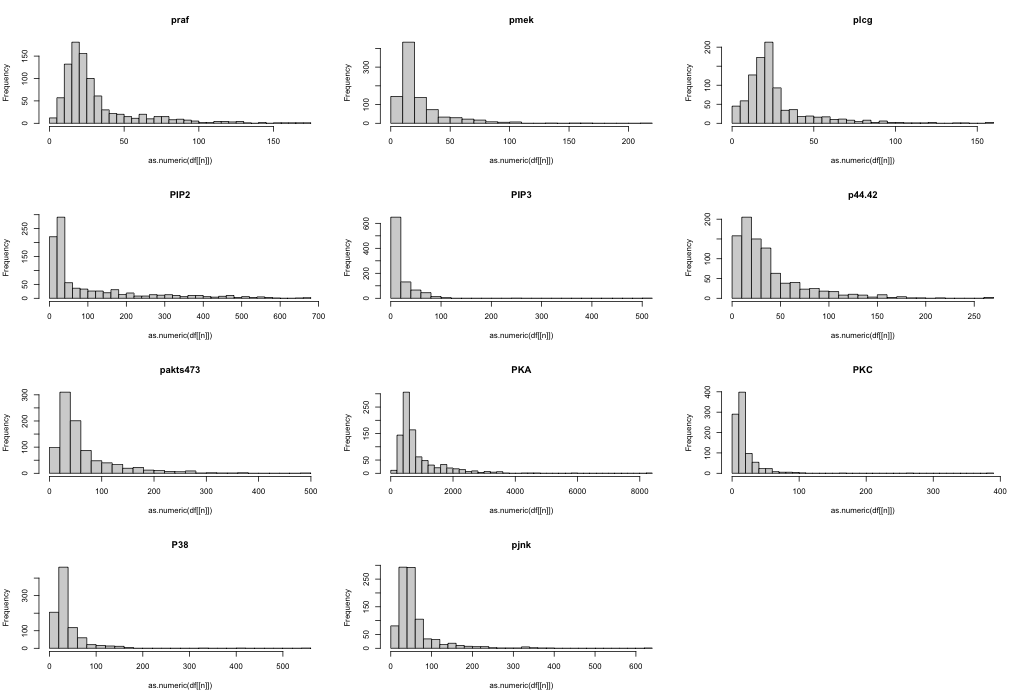
\includegraphics{data/distribution_plots/original/pma.png} and we can
simply understand that our data is all but normally distributed. Just to
be sure, we ran boxplots and Shapiro-tests that confirmed our
hypothesis.

Our intention was then to modify the data in order to approximate a
zero-mean Gaussian. We tried different methodologies such as scale
method, subtract the mean and divide by the standard deviation and
box-cox. We opted for a combination of a box-cox transformation and
scale method. The box-cox transformation is implemented as:
\begin{equation}
y(\lambda)= 
\begin{cases}
    \frac{y^{\lambda}-1}{\lambda},& \text{if } \lambda \neq 0\\
    log(y),              & \text{if} \lambda = 0
\end{cases}
\end{equation}

in code we have:

\begin{Shaded}
\begin{Highlighting}[]
\NormalTok{boxcox.transform=}\StringTok{ }\ControlFlowTok{function}\NormalTok{(data)\{}
\NormalTok{  bx =}\StringTok{ }\KeywordTok{boxcox}\NormalTok{(data}\OperatorTok{~}\DecValTok{1}\NormalTok{, }\DataTypeTok{plotit =}\NormalTok{ F)}
\NormalTok{  lambda =}\StringTok{ }\NormalTok{bx}\OperatorTok{$}\NormalTok{x[}\KeywordTok{which}\NormalTok{(bx}\OperatorTok{$}\NormalTok{y}\OperatorTok{==}\KeywordTok{max}\NormalTok{(bx}\OperatorTok{$}\NormalTok{y))[}\DecValTok{1}\NormalTok{]]}
  \ControlFlowTok{if}\NormalTok{(lambda }\OperatorTok{!=}\StringTok{ }\DecValTok{0}\NormalTok{)}
    \KeywordTok{return}\NormalTok{((data}\OperatorTok{^}\NormalTok{lambda}\DecValTok{-1}\NormalTok{)}\OperatorTok{/}\NormalTok{lambda)}
  \ControlFlowTok{else}
    \KeywordTok{return}\NormalTok{(}\KeywordTok{log}\NormalTok{(data))}
\NormalTok{\}}
\NormalTok{normalize =}\StringTok{ }\ControlFlowTok{function}\NormalTok{(data)}
  \KeywordTok{return}\NormalTok{(}\KeywordTok{scale}\NormalTok{(}\KeywordTok{boxcox.transform}\NormalTok{(data)))}
\end{Highlighting}
\end{Shaded}

After applying this transformation to our data, we ended out with this
result: we can see green histograms after the process of scaling and
soft blue histogram after the boxcox transformation.
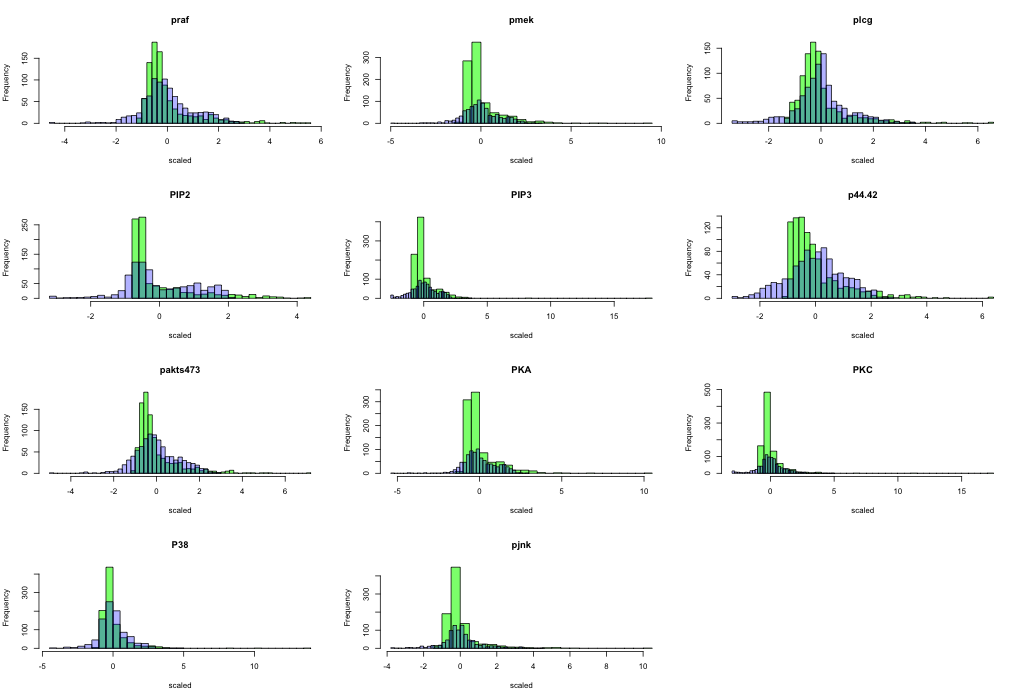
\includegraphics{data/distribution_plots/scaled_vs_normalized/pma.png}

This seems a good result starting from our data: in fact, they
graphically appear normally distributed around 0.

\hypertarget{connection-1-pip2-pkc-pareggio}{%
\subsubsection{CONNECTION 1 PIP2-\textgreater PKC \#
pareggio}\label{connection-1-pip2-pkc-pareggio}}

We fixed a level alpha=0.05 so that we have
\(log(\frac{1}{\alpha})\simeq2.99\). The following table summarizes our
results.

\begin{longtable}[]{@{}lrcc@{}}
\toprule
k & pvalue\_MLE\_dag & log(Un) & log(Wn)\tabularnewline
\midrule
\endhead
0.01 & 1 & -16.19 & -15.48,\tabularnewline
0.1 & 1 & -16.19 & -15.48,\tabularnewline
1 & 0.21 & -18.48 & -14.64\tabularnewline
10 & 0.21 & -18.48 & -14.64\tabularnewline
100 & 0.21 & -18.48 & -14.64\tabularnewline
\bottomrule
\end{longtable}

They did not reject the null hypothesis and we can confirm that it is a
missed linkage. Similarly, our test was not able to reject the null
hypothesis. The sparsity parameter K did not have a strong impact on the
results

\hypertarget{second-connection-pkc-jnk-cuxe9-male}{%
\subsubsection{SECOND CONNECTION: PKC-\textgreater Jnk \# C'é
\#male}\label{second-connection-pkc-jnk-cuxe9-male}}

\begin{longtable}[]{@{}lrcc@{}}
\toprule
k & pvalue\_MLE\_dag & log(Un) & log(Wn)\tabularnewline
\midrule
\endhead
0.01 & 1 & -16.19 & -15.48\tabularnewline
0.1 & 1 & -16.19 & -15.48\tabularnewline
1 & 6.0e-11 & 17.05 & 16.36\tabularnewline
10 & 6.0e-11 & 17.05 & 16.36\tabularnewline
100 & 6.0e-11 & 17.05 & 16.36\tabularnewline
\bottomrule
\end{longtable}

In this case, we need to notice the strong influence of k parameter on
the results: we can not say a priori when we reject or accept the null
hypothesis and an image should help to understand the behavior of our
statistics when the k parameter changes. Our tests seem to have similar
results as MLEdag

\begin{figure}
\centering
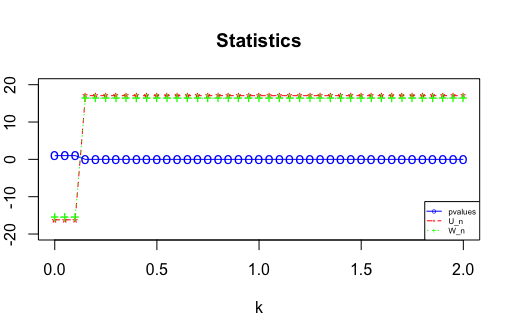
\includegraphics{data/statistics_images/Part5.2.png}
\caption{statistiche}
\end{figure}

\hypertarget{third-connection-pkc-pip3-non-cuxe8-bene2}{%
\subsubsection{THIRD CONNECTION: PKC-\textgreater PIP3 \# Non c'è
\#bene*2}\label{third-connection-pkc-pip3-non-cuxe8-bene2}}

\begin{longtable}[]{@{}lrcc@{}}
\toprule
k & pvalue\_MLE\_dag & log(Un) & log(Wn)\tabularnewline
\midrule
\endhead
0.01 & 1 & -16.19 & -15.48\tabularnewline
0.1 & 0.60 & -15.80 & -14.80\tabularnewline
1 & 0.60 & -15.80 & -14.80\tabularnewline
10 & 0.60 & -15.80 & -14.80\tabularnewline
100 & 0.60 & -15.80 & -14.80\tabularnewline
\bottomrule
\end{longtable}

In this case the tests are equivalent: MLEdag correctly accepts the null
hypothesis and we did the same. The k parameter did not have a central
role in this test with a exception of k=0.01 in which MLE\_dag as a
p-value=1

\#PATHWAY LINKAGE: PKC-\textgreater(RAF;MEK,ERK) \#male*2

\begin{longtable}[]{@{}lrcc@{}}
\toprule
k & pvalue\_MLE\_dag & log(Un) & log(Wn)\tabularnewline
\midrule
\endhead
0.01 & 0.82 & -71.56 & -56.09\tabularnewline
0.1 & 0.82 & -71.56 & -56.09\tabularnewline
1 & 1.62e-106 & -71.56 & -56.09\tabularnewline
10 & 1.62e-106 & -71.56 & -56.09\tabularnewline
100 & 1.62e-106 & -71.56 & -56.09\tabularnewline
\bottomrule
\end{longtable}

This is a interesting simulation: our statistics log(Un) and log(Wn) had
a stable result as the k parameter changed. On the other hand MLE\_dag
produces contrasting p-values. Also in this situation an image should
help to understand the fluctuation.
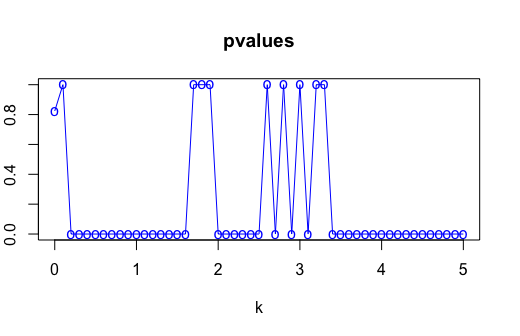
\includegraphics{data/statistics_images/Part5.4.png}

As a final remark, we need to notice that we have used a dataset in
which there was a perturbation on PKC that should be responsible of
these results. Consequently, we need to pay attention to the conclusion
based on the whole dataset: will the results be the same?

\hypertarget{point-6}{%
\subsection{POINT 6}\label{point-6}}

Now let's move on the entire dataset obtained concatenating all the
data. As before, we can visually check our zero-mean Gaussian
aasumptions.

This is our starting point
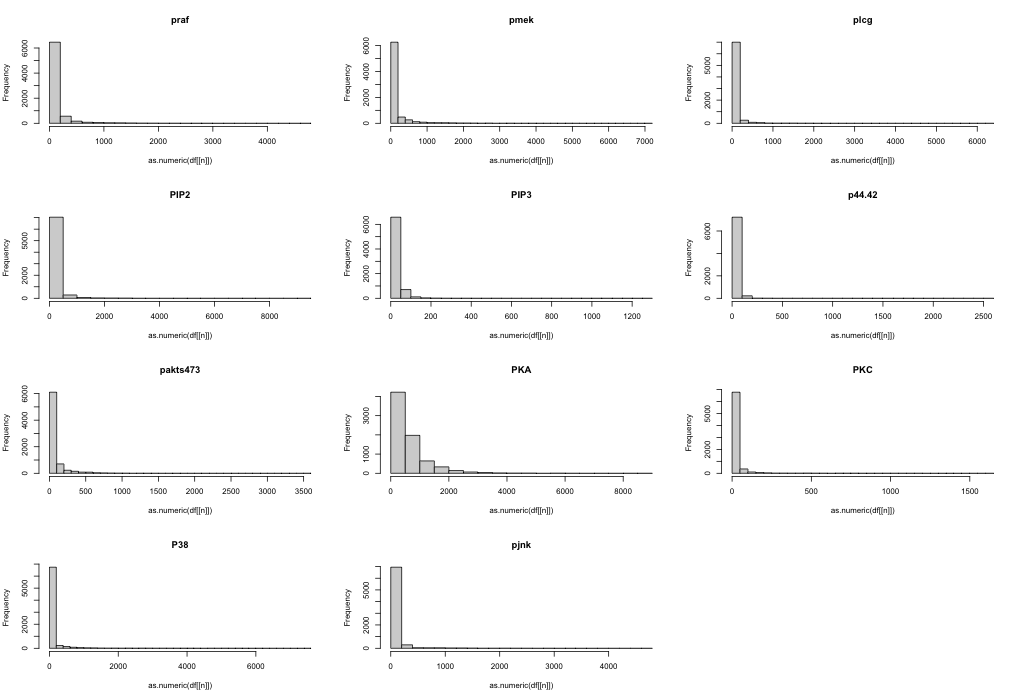
\includegraphics{data/distribution_plots/original/concatenated.png} and
after our transformation (box-cox and scale ), we have
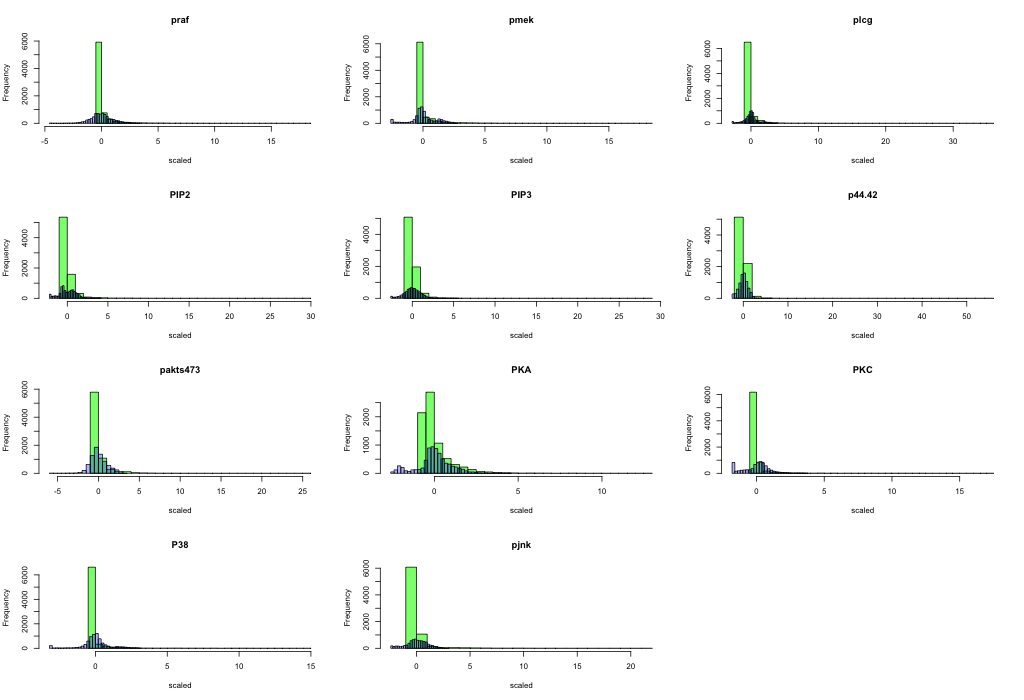
\includegraphics{data/distribution_plots/scaled_vs_normalized/concatenated.png}
As before, we can say that we achieved a good result with respect to our
assumption. It's interesting to compare the results of our test on a
different dataset in which we find different kinds of perturbations.

We fixed a level alpha=0.05 so that we have \$
log(\frac{1}{\alpha})\simeq1.30 \$. The following table summarizes our
results.

\hypertarget{connection-1-pip2-pkc-pareggio-1}{%
\subsubsection{CONNECTION 1 PIP2-\textgreater PKC \#
pareggio}\label{connection-1-pip2-pkc-pareggio-1}}

We fixed a level alpha=0.05 so that we have
\(log(\frac{1}{\alpha})\simeq1.30\). The following table summarizes our
results.

\begin{longtable}[]{@{}lrcc@{}}
\toprule
k & pvalue\_MLE\_dag & log(Un) & log(Wn)\tabularnewline
\midrule
\endhead
0.01 & 1 & -625.26 & -534.54\tabularnewline
0.1 & 1 & -625.26 & -534.54\tabularnewline
1 & 1 & -466.80 & -407.60\tabularnewline
10 & 1 & -466.80 & -407.60\tabularnewline
100 & 1 & -625.26 & -534.54\tabularnewline
\bottomrule
\end{longtable}

They did not reject the null hypothesis, but we got the same results.

\hypertarget{second-connection-pkc-jnk-cuxe9-male-1}{%
\subsubsection{SECOND CONNECTION: PKC-\textgreater Jnk \# C'é
\#male}\label{second-connection-pkc-jnk-cuxe9-male-1}}

\begin{longtable}[]{@{}lrcc@{}}
\toprule
k & pvalue\_MLE\_dag & log(Un) & log(Wn)\tabularnewline
\midrule
\endhead
0.01 & 0 & -297.12 & -297.81\tabularnewline
0.1 & 0 & -297.12 & -297.81\tabularnewline
1 & 0 & 36.50 & 35.81\tabularnewline
10 & 0 & -297.12 & -297.81\tabularnewline
100 & 0 & -297.12 & -297.81\tabularnewline
\bottomrule
\end{longtable}

In this case, we need to notice the strong influence of k parameter on
our statistics as in point five: we ended up witha wrong conclusion in
all the cases expect for k=1.

\begin{figure}
\centering
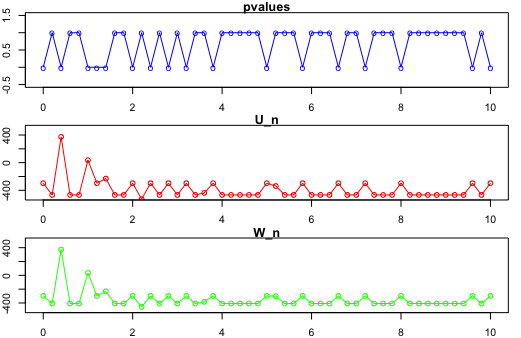
\includegraphics{data/statistics_images/Part6.2.png}
\caption{statistiche}
\end{figure}

\hypertarget{third-connection-pkc-pip3-non-cuxe8-bene2-1}{%
\subsubsection{THIRD CONNECTION: PKC-\textgreater PIP3 \# Non c'è
\#bene*2}\label{third-connection-pkc-pip3-non-cuxe8-bene2-1}}

\begin{longtable}[]{@{}lrcc@{}}
\toprule
k & pvalue\_MLE\_dag & log(Un) & log(Wn)\tabularnewline
\midrule
\endhead
0.01 & 1 & -625.26 & -534.54\tabularnewline
0.1 & 1 & -625.26 & -534.54\tabularnewline
1 & 1 & -466.80 & -407.60\tabularnewline
10 & 0.84 & -585.54 & -504.55\tabularnewline
100 & 1 & -625.26 & -534.54\tabularnewline
\bottomrule
\end{longtable}

In this case the test are equivalent: MLEdag accepts correctly the null
hypothesis and we did the same. The k parameter did not have a central
role in this test with the exception of the values k=1 and k=10

\#PATHWAY LINKAGE: PKC-\textgreater(RAF;MEK,ERK)

\begin{longtable}[]{@{}lrcc@{}}
\toprule
k & pvalue\_MLE\_dag & log(Un) & log(Wn)\tabularnewline
\midrule
\endhead
0.01 & 1 & -924.26 & -Inf\tabularnewline
0.1 & 1 & -924.26 & -Inf\tabularnewline
1 & 0 & -924.26 & -Inf\tabularnewline
10 & 0 & -924.26 & -Inf\tabularnewline
100 & 0 & -924.26 & -Inf\tabularnewline
\bottomrule
\end{longtable}

This is an interesting simulation: our statistics log(Un) and log(Wn)
had a stable result as the k parameter changed. On the other hand
MLE\_dag produces contrasting pvalues. This is another case where an
image should help understanding the fluctuation:

\begin{figure}
\centering
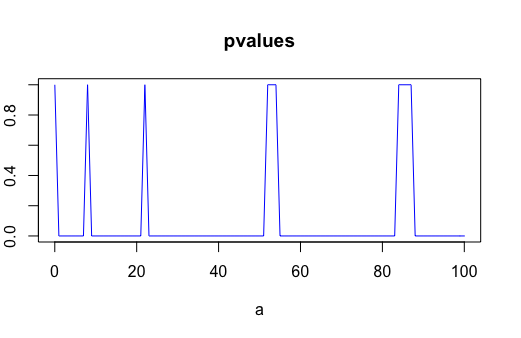
\includegraphics{data/statistics_images/Part6.4.png}
\caption{statistiche}
\end{figure}

\#CONCLUSIONI

\hypertarget{domande}{%
\subsubsection{DOMANDE}\label{domande}}

Regarding adjusting for multiplicity, we feel it could be a sensible
choice in our case: while testing our pathway-type hypothesis, we are
dealing with the intersection of different events, and, if we want to
check for a path between the element 1, 2 and 3, we need to check if
there's a link between 1 and 2, and then between 2 and 3. This means
that for every single link we are searching has an alpha level of false
rejection risk associated to it, and adjusting for multiplicity (via
Bonferroni's method or others) could prove to be useful in avoiding a
pretty high risk of false rejection, since as we know the probability of
a Type I error in multiple tests is \(P= 1-(1-\alpha)^{k}\), where alpha
is our significance level and k is the number of tests we are
performing. Adjusting for multiplicity could also prove to be useful in
the linkage case: while we aren't performing multiple test in this
homework, testing our linkages one-by-one, one could carry out their
analysis on a set F, in which case adjusting for multiplicity could
prove to be useful, if not downright needed.

\begin{itemize}
\item
\end{itemize}

\end{document}
